\documentclass[11pt,english]{article}
\usepackage{amssymb}
\usepackage{siunitx}
\usepackage{tikz}
\usepackage{subcaption}
\usepackage{float} % pour [H] si besoin
\usetikzlibrary{arrows.meta, positioning, graphs}

\usepackage[T1]{fontenc}
\usepackage[margin = 0.7in, includefoot]{geometry}
\def\changemargin#1#2{\list{}{\rightmargin#2\leftmargin#1}\item[]}
\let\endchangemargin=\endlist 
\usepackage[utf8]{inputenc}
\usepackage{babel}
\usepackage{float}
\usepackage{xcolor}
\usepackage{amsmath}
\usepackage{csquotes}
\usepackage{hyperref}
\hypersetup{
	colorlinks=true,
	urlcolor=magenta,
    citecolor=blue,
	linkcolor=magenta,
	breaklinks=true
}

\usepackage{listings}
\lstdefinestyle{cstyle}{
    language=C,
    basicstyle=\ttfamily\small,
    keywordstyle=\color{blue}\bfseries,
    stringstyle=\color{red!60!black},
    commentstyle=\color{green!50!black}\itshape,
    numberstyle=\tiny\color{gray},
    numbers=left,
    stepnumber=1,
    numbersep=8pt,
    tabsize=2,
    showspaces=false,
    showstringspaces=false,
    showtabs=false,
    frame=single,
    rulecolor=\color{black!30},
    breaklines=true,
    breakatwhitespace=true,
    captionpos=b,
    keepspaces=true,
    columns=fullflexible,
    upquote=true
}

\lstset{style=cstyle}

\usepackage{graphicx} % Required for inserting images
\usepackage{grffile}
\usepackage[numbib] {tocbibind}
\usepackage{datetime}
\parskip=2mm
\parindent=0mm

\begin{document}


%%%%%%%%%%%%%%%%%%%%%%%%%%%%%%%%%%%%%%%%%%%%%%%%%%%%%%%%%%%%%%%%%%%%%%%%%%%%%%
% Page de garde
%%%%%%%%%%%%%%%%%%%%%%%%%%%%%%%%%%%%%%%%%%%%%%%%%%%%%%%%%%%%%%%%%%%%%%%%%%%%%%
\thispagestyle{empty}

\begin{center}
    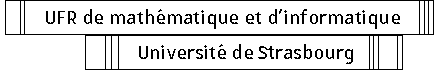
\includegraphics[width=9cm] {assets/img/logo-ufr.pdf}       

    \vfill

    {
	\large
    	\textsc{
    	    CMI d'informatique \\
    	    Cursus Master en Ingénierie en Informatique, Systèmes et Réseaux
    	}
    }

    \bigskip\bigskip
    \bigskip\bigskip

    {\huge Travail d’Étude et de Recherche (TER)}

    \bigskip\bigskip

    % Identité des auteurs
    {\large Jeronimo \textsc{Herdoïza}} \\

    \medskip
    
    % Contacter les auteurs
    {\small jeronimo.herdoiza@etu.unistra.fr}

    \vfill

    {
	\Huge
    	\textsc{
    	    Thread Scheduling for Transformers\\
    	}
    }
    

    \vfill
    \vfill

    \newdate{date}{03}{05}{2026}
    \displaydate{date}

    \vfill

    {\large Research work supervised by}

    \medskip

    % Identité de l'encadrant
    {\large Cedric \textsc{Bastoul}}\\

    % Contact mail ou téléphone
    {\small  bastoul@unistra.fr }

    \bigskip
    \bigskip
\end{center}

\clearpage



\tableofcontents

\clearpage

\section{Introduction}
\section{Background}
\section{State of the art}
    \subsection{Thread Scheduling in Parallel Computing}

    Thread scheduling has been a fundamental problem im parallel computing since several decades: given a set of computations and a fixed number of CPU cores, the scheduler has to decide which thread runs on which core at which time. As of today, where multicore architecures have become the norm, these decisions have a critical impact on load balance, cache utilization, memory locality, and synchronization overhead. To address this problem, two main families of scheduling policies have been found to be effective: \emph{work sharing} and \emph{work stealing}.

    \subsection{Work Sharing}

    With \emph{work sharing} when new work is created, the scheduler assigns the tasks among the available worker threads. This approach is rather simple but can lead to poor load balance when the cost of iterations varies significantly, this is due to the fact that the work distribution is set before the loop begins and cannot be adjusted at runtime.

    OpenMP is the most widely used API in this domain~\cite{mishra2024cows}. It provides several clauses that aim to avoid this problem and improve load balance. For instance, the \texttt{dynamic} clause allows the scheduler to assign iterations to threads dynamically as they become available. The \texttt{guided} clause works in a similar way but executes large chunks of iterations at the beginning of the loop and decrease the size of these chunks as the loop progresses. Finally, the \texttt{static} clause works the way described above, in most implementations of OpenMP, this is the default scheduling policy.

    \subsection{Work Stealing}

    \emph{Work stealing} was formalized by Blumofe and Leiserson~\cite{blumofe1999workstealing} in 1999. They take a different approach than work sharing: rather than pushing work from a central source, idle threads will pull tasks from other busy threads. This means that all threads have their own double-ended queue (deque). Inside each thread, tasks first treated in a LIFO order to preserve locality and cache reuse, on the other hand, thieves will come and steal from the oposite end of the deque (FIFO).

    Blumofe and Leiserson proved that on $P$ processors, the expected execution time of a fully strict multithreaded computation under work stealing satisfies:
    \[
        T_P \leq \frac{T_1}{P} + O(T_\infty)
    \]
    where $T_1$ is the serial execution time and $T_\infty$ is the critical-path length with unlimited processors. Space usage is bounded at $S_1 P$, and expected total communication at $O(PT_\infty(1 + n_d)S_{\max})$, where $S_{\max}$ is the size of the largest activation record and $n_d$ is the maximum thread synchronization depth. This communication bound formally justifies the intuition that work-stealing schedulers are more efficient than work-sharing counterparts: stolen tasks are coarse-grained and steals are rare in balanced workloads~\cite{blumofe1999workstealing}.

    The work by Blumofe and Leiserson~\cite{blumofe1999workstealing} made work stealing widely adopted in parallel programming. For instance OpenMP implemented work stealing in its task clause. However, this implementation is not standardized in the API and varies significantly among different runtimes, making it difficult to reason about or tune for a specific workload.

    \subsection{Advanced Scheduling Variants}
    Several variants of work stealing have been proposed in the literature because of the limitations of the original scheme. Especially in the context of Non Uniform Memory Access (NUMA) architectures, such as the ones studied in this work, where stealing from a remote thread can be costly. This has motivated the design of NUMA-aware work stealing and other scheduling strategies.

    \paragraph{Cost-Aware Work Stealing (COWS).}
    Mishra and Nandivada~\cite{mishra2024cows} identify three fundamental shortcomings when work stealing is applied to parallel-for loops:  
    \begin{itemize}
        \item not all iterations take the same time, this means that stealing a fixed number of iterations will not equalize the load,
        \item selecting a suitable victim is non-trivial, and selecting one randomly performs poorly,
        \item the per-thread deque required by traditional work stealing introduces overhead that exceeds its benefit for moderately irregular loops.
    \end{itemize}
    Their scheme addresses all three simultaneously.

    COWS proposes two variants. Work Stealing based on Remaining Iterations (\emph{WSRI}) tracks the number of remaining iterations for each thread in a lightweight shared scalar, replacing the deque entirely, and uses this information to select the most loaded victim. Work Stealing based on Remaining Workload (\emph{WSRW}) uses a compile-time analysis to emit application-specific instrumentation code, enabling the runtime to estimate the remaining computational cost of each thread rather than merely its iteration count. In 225 out of 275 tested configurations spanning 7 benchmarks, 5 datasets, and 2 hardware platforms, COWS outperforms the best available OpenMP scheduling scheme, with clear advantages for power-law graph workloads where static and dynamic schedules both fail~\cite{mishra2024cows}.

    \paragraph{NUMA-Aware and Distance-Aware Work Stealing.}    
    It's well known in systems programming that memory accesses are costly. On NUMA architectures, a naive implementation of work stealing can lead to significant performance issues due to this issue. Indeed, when a thread steals a task from a remote NUMA node, it may move the task far from its data and cause repeated remote memory accesses for the stolen task's entire execution.

    Applied to Cholesky factorization and symmetric matrix inversion on a large NUMA system, this approach achieves up to a twofold speedup in flop rate over non-discriminating policies and matches or exceeds the performance of state-of-the-art commercial and open-source HPC libraries~\cite{alomairy2015numa}. The key insight is that on modern hardware, the scheduler must treat the memory topology of the machine as a first-class input to its decision-making, not an afterthought.

    Al-Omairy et al.~\cite{alomairy2015numa} address this with a \emph{distance-aware} scheduling policy built on the OmpSs task-based programming model. The key insight for their scheduler must treat the memory topology of the machine as a critical input to its decision-making, not as a secondary concern. They approach the scheduling in a topology-aware manner. For instance, a thief will prefer to steal from its nearest NUMA neighbor, making the decision to go for more distant nodes exclusively when local work is exhausted. When applied to Cholesky factorization and symmetric matrix inversion on a large NUMA system, the results show up to a twofold speedup, matching or exceeding the performance of state-of-the-art commercial and open-source HPC libraries~\cite{alomairy2015numa}.

    \subsection{Transformer Inference on CPUs}

    \paragraph{Computational structure of Transformers.}
    Transformer models are composed of stacked encoder and/or decoder layers, each containing a \emph{multi-head self-attention} sublayer and a \emph{position-wise feed-forward} sublayer. The attention mechanism computes:
    \[
        \text{Attn}(Q, K, V) = \text{softmax}\!\left(\frac{QK^T}{\sqrt{d_k}}\right)V
    \]
    and the multi-head variant concatenates $h$ such heads, requiring 3 matrix multiplications for the $Q$, $K$, $V$ projections plus 2 batched matrix multiplications for the attention scores and weighted sum~\cite{dice2021transformercpu}. The feed-forward sublayer contributes two further large matrix multiplications. In total, general matrix multiplication (GEMM) is the dominant computation in Transformer inference, typically accounting for 70--90\% of total runtime~\cite{dice2021transformercpu}, making it the primary target for parallelization and scheduling optimization.

    \paragraph{Optimizing Transformer inference on CPUs.}
    Dice and Kogan~\cite{dice2021transformercpu} conduct an empirical analysis of Transformer (BERT) inference on Intel Skylake CPUs with the oneDNN/MKL-DNN math library. They identify three orthogonal bottlenecks. First, matmul performance depends critically on whether source matrices are provided in transposed form; the wrong choice incurs substantial overhead. They propose an adaptive selection mechanism for the optimal matrix layout at runtime. Second, each individual matmul call in deep-learning frameworks carries a \emph{sequential invocation overhead} from thread pool dispatch and kernel setup that is independent of matrix size and degrades scalability at small batch sizes. Third, the sub-matrix partitioning for inner kernels may be suboptimal relative to cache capacity, causing unnecessary cache misses. Their combined optimizations yield up to 2.37$\times$ speedup on BERT without any model change. This work directly motivates the parallelization strategy adopted in this report: since GEMM dominates, thread-level parallelism must carefully account for per-call overhead.
 
    \paragraph{Transformer inference on ARM many-core processors.}
    Jiang et al.~\cite{jiang2022arm} characterize and optimize Transformer inference specifically on ARM many-core CPUs, which share structural properties with the Snapdragon SoC used in this work. They identify three bottleneck categories: suboptimal thread scheduling and configuration, GEMM implementations that ignore the irregular shapes of Transformer attention matrices, and redundant computations from padding-based batching. To address scheduling, they design a \emph{NUMA-aware thread scheduling} policy paired with a lookup table that maps workload configurations to optimal thread counts, avoiding the performance cliff that emerges when thread count exceeds the L3 bandwidth saturation point. For GEMM, they tailor kernels to the shapes of self-attention and feed-forward projections using ARM SIMD instructions, and introduce a sparse data format for variable-length inputs. Their implementation outperforms PyTorch and TurboTransformer by 1.1$\times$--6$\times$ on fixed-length inputs and up to 6$\times$ on variable-length inputs, demonstrating that holistic, architecture-aware optimization at both the operator and scheduling level is essential for Transformer inference on ARM platforms.
 
    \subsection{Lock-Free and Scalable Work Stealing}
 
    A persistent practical challenge for work stealing at high thread counts is the overhead of the concurrent data structures that manage the deques and coordinate steals. Traditional implementations rely on mutex locks or compare-and-swap (CAS) operations, which cause cache-coherence traffic that grows super-linearly with thread count.
 
    Yang and He~\cite{yanghe2018survey} survey the evolution of work-stealing algorithms and implementations along three axes: scheduling algorithm design, data structure optimizations, and processor-architecture-oriented techniques. They observe that on heterogeneous platforms, including ARM big.LITTLE architectures, naive work stealing that treats all processors as equivalent yields poor results, because stealing from a slow core transfers work that will take disproportionately long to complete. Architecture-aware variants incorporating processor speed or memory locality into victim selection and steal granularity are identified as a key open research direction.
 
    Nookala et al.~\cite{nookala2024xopenmp} address the synchronization bottleneck directly with X-OpenMP, extending the OpenMP tasking model with a lock-\emph{less} work stealing algorithm built on the XQueue structure. XQueue uses relaxed memory ordering (store-release/load-acquire) to avoid mutual exclusion or CAS, which are natively cheap on modern out-of-order processors. On many-core systems with up to 384 hardware threads across Intel, AMD, IBM, and ARM platforms, X-OpenMP achieves up to 40$\times$ speedup over GNU OpenMP and reduces tasking overhead by 50\%. The key insight is that the centralized queue of OMP \texttt{dynamic} scheduling becomes a hard scalability bottleneck at high concurrency due to atomic fetch-and-add contention, confirming the theoretical advantage of decentralized work stealing.
 
    \subsection{Fine-Grained NUMA-Aware Scheduling}
 
    Hu et al.~\cite{hu2023find} introduce FinD, a fine-grained dynamic task scheduling framework for many-core processors. FinD operates on lightweight user-level threads (via the Argobots library) rather than kernel threads, eliminating context-switching overhead. The key scheduling contribution is a \emph{bilateral NUMA-aware work stealing} mechanism: both the thief and the victim cooperate to select the optimal task from the nearest NUMA node, substantially reducing remote memory access latency. FinD additionally introduces a main/secondary task pool architecture based on double-ended queues, enabling fine-grained dynamic load balancing without per-task deque management overhead. Evaluation on an ARM many-core cluster shows up to 9.7$\times$ speedup over popular data frameworks on HPC workloads and 40\% reduction in execution time on skewed datasets. FinD illustrates that on ARM many-core platforms, the design of the deque and the NUMA-awareness of victim selection have first-order impact on performance --- a principle directly applicable to the heterogeneous Snapdragon SoC targeted in this work.


\section{Implementation}

Work sharing implementation with \texttt{OpenMP} was already implemented in the \texttt{StrasGPT} codebase during the \"Parallel Programming\" course in autumn semester. The implementation targets the same transformer inference parallelization on shared-memory multicore processors, this includes heterogenous architectures such as ARM big.LITTLE. This work main contribution is a custom work stealing scheduler designed specifically to address this computational structure. The scheduler is implemented in C and integrates into the existing codebase via conditional compilation (\texttt{-DWS\_SCHEDULER=1}).
 
\subsection{Parallelization Targets in Transformer Inference}
 
Before describing scheduling decisions, it is necessary to identify which operations are parallelized. Following the analysis by Dice et al.~\cite{dice2021transformercpu}, general matrix multiplication (GEMM) is the dominant operation, accounting for 70--90\% of inference time. In \texttt{StrasGPT}, the following operations within each decoder layer are parallelized across worker threads:
 
\begin{itemize}
    \item \textbf{Key and Value projection matmuls} (\texttt{ws\_attn\_kv\_matmul}): for each KV-head $k$ and token $t$, a dot product of size $d_{\text{emb}}$ is computed. The iteration space is flattened to $n_{\text{kv}} \times T \times d_{\text{head}}$ scalar tasks.
    \item \textbf{Query projection matmul} (\texttt{ws\_attn\_q\_matmul\_worker}): similarly flattened over $n_{\text{kv}} \times q_{\text{per\_kv}} \times T \times d_{\text{head}}$ tasks, accounting for the Grouped Query Attention (GQA) head structure.
    \item \textbf{Multi-head attention} (\texttt{ws\_attn\_worker}): each task computes a full $\text{QK}^\top$, a numerically stable softmax, and the weighted sum over $V$ for a single (KV-head, Q-head, token) triplet. This kernel has \emph{variable} computational cost proportional to $s = \text{cached\_count} + t + 1$, which grows with sequence length and renders static partitioning suboptimal.
    \item \textbf{FFN matmuls} (\texttt{ws\_matmul\_row}): the feed-forward sublayer's three linear projections are parallelized row-by-row over the output dimension.
    \item \textbf{Logit projection}: the final vocabulary classifier is parallelized over $\text{logits\_count} \times |\mathcal{V}|$ tasks.
\end{itemize}
 
The remaining operations (residual connections, layer normalization, etc.) are not parallelized with work stealing due to their lower computational intensity and the overhead of task management.

\noindent Each parallelized kernel is exposed to the scheduler as a contiguous integer range $[\text{begin}, \text{end}]$ of independent tasks, with an associated callback function following the signature \texttt{void fn(int64\_t i, void *arg)}.
 
\subsection{The Work-Stealing Scheduler: \texttt{ws\_scheduler}}
 
\subsubsection{Task Representation: Ranges Rather Than Individual Iterations}
 
A fundamental design decision is the granularity of tasks placed on the deques. Two extreme choices are:
\begin{enumerate}
    \item Enqueue individual iterations, incurring per-iteration synchronization overhead;
    \item Enqueue a single coarse task per worker, yielding no dynamic rebalancing capability.
\end{enumerate}
 
The implementation adopts an intermediate \emph{range-based} task representation: each deque entry is a \texttt{ws\_range\_t}, a pair \texttt{(begin, end)} encoding a contiguous sub-interval of the iteration space. This is consistent with the observation by Traor\'e et al.~\cite[Ref.~56]{yanghe2018survey} that independent tasks can be compactly represented by index ranges, avoiding per-task allocation overhead. Each worker is initially assigned a single range covering its entire allocated slice; if a thief steals this range, it executes the stolen interval atomically, and subsequently attempts to steal further work if it remains idle. The deque capacity is fixed at 4096 entries (\texttt{WS\_DEQUE\_CAP}), which is amply sufficient given that each worker holds at most one range at initialization.
 
\subsubsection{The Lock-Free Double-Ended Queue: Chase--Lev Deque}
 
The per-worker task queue implements the \emph{Chase--Lev} dynamic circular work-stealing deque~\cite{chaselev2005deque}, which is the standard lock-free deque used in production work-stealing runtimes such as Cilk. It provides:
 
\begin{itemize}
    \item \textbf{Owner operations} (\texttt{deque\_push}, \texttt{deque\_pop}): the owning thread pushes and pops from the \emph{bottom} end of the deque in LIFO order. These operations are wait-free for the owner in the non-contended case.
    \item \textbf{Steal operation} (\texttt{deque\_steal}): thieves steal from the \emph{top} end of the deque in FIFO order. A \texttt{compare\_exchange\_strong} on the \texttt{top} atomic counter resolves races between concurrent thieves and a concurrent \texttt{deque\_pop} on the last element.
\end{itemize}
 
The memory ordering discipline is as follows. \texttt{deque\_push} uses a \texttt{memory\_order\_release} store on \texttt{bottom} to make the newly written buffer slot visible to thieves. \texttt{deque\_pop} uses a sequentially consistent fence (\texttt{memory\_order\_seq\_cst}) to synchronize with concurrent steals on the last element, as required by the THE protocol by Frigo et al.~\cite[Ref.~2]{yanghe2018survey}. \texttt{deque\_steal} uses \texttt{memory\_order\_acquire} loads on both \texttt{top} and \texttt{bottom} to observe the owner's most recent push, followed by a \texttt{memory\_order\_seq\_cst} CAS on \texttt{top}. This ordering ensures correctness on the relaxed memory models found on ARM architectures targeted by the Android deployment (Lê et al.~\cite[Ref.~55]{yanghe2018survey}).
 
The LIFO ordering for the owner is critical for cache performance: the most recently pushed range is the one whose data is most likely still resident in L1/L2 cache. Thieves, conversely, steal from the opposite end, obtaining the oldest (largest) available range, which minimizes the number of steals required to balance the load as stated by Blumofe and Leiserson~\cite{blumofe1999workstealing}.
 
\subsubsection{Heterogeneity-Aware Initial Partitioning}
 
On big.LITTLE processors (e.g., the Qualcomm Snapdragon 8 gen 2 for Galaxy in figure~\ref{fig:snapdragon}, which is a primary deployment target), performance cores (big) and efficiency cores (LITTLE) operate at significantly different clock frequencies. A uniform partition that assigns $N/P$ iterations to each of $P$ workers would systematically overload the efficiency cores and leave the performance cores underutilized.
 
To address this, the scheduler implements a \emph{weighted initial partition} inspired by the cost-aware scheduling philosophy of COWS~\cite{mishra2024cows}. At initialization, \texttt{ws\_ctx\_init} reads the maximum CPU frequency of each core from the Linux sysfs interface (\texttt{/sys/devices/system/cpu/cpuN/
cpufreq/cpuinfo\_max\_freq}) and assigns a weight $w_i \in \{1, 2, 4\}$ proportional to frequency tier (below 2.5~GHz, 2.5--3~GHz, or above 3~GHz). Thread 0 then distributes the iteration range such that worker $i$ receives a fraction $w_i / \sum_j w_j$ of the total work. Each worker's share is pushed as a single range onto its deque, and its \texttt{remaining} counter is set accordingly.
 
The weighted partition reduces the expected number of steals in the common case by making the initial distribution already well-balanced, thereby limiting the synchronization overhead that would otherwise be incurred by extensive stealing from slower cores. This only in Linux-based systems, in other operating systems suc as MacOS, the scheduler falls back to a uniform partition since core frequency information is not exposed to user-space applications, we assume cores are homogeneous in this case.
 
\subsubsection{Victim Selection Strategy}
 
When a worker exhausts its local deque, it enters the \emph{stealing loop} and must select a victim. Two strategies are implemented and selected based on whether a cost function was supplied:
 
\paragraph{Randomized victim selection.} In the absence of a cost function, a victim is chosen uniformly at random among all workers other than the thief, using a local \emph{xorshift64} PRNG seeded per-thread. This recovers the classical randomized work-stealing algorithm of Blumofe and Leiserson~\cite{blumofe1999workstealing}, for which the expected execution time satisfies $T_P \leq T_1/P + O(T_\infty)$.
 
\paragraph{Cost-aware victim selection (WSRI-style).} When a \texttt{ws\_cost\_fn} callback is provided, thread 0 pre-computes a prefix-sum array over the iteration costs before distributing work. In the stealing loop, the thief scans all workers and selects the one with the highest \texttt{remaining} counter (loaded with \texttt{memory\_order\_relaxed} to avoid costly acquire fences). This implements the WSRI strategy of Mishra and Nandivada~\cite{mishra2024cows}, where the victim is the most loaded worker rather than a random one, improving load balance for highly irregular workloads. For the multi-head attention kernel, whose per-task cost increases monotonically with sequence position $s$, this strategy is particularly beneficial.
 
\paragraph{Termination detection.} After a failed steal, the thief performs a full scan of all \texttt{remaining} counters. If all are zero, the stealing loop terminates. Otherwise, the thief yields via \texttt{sched\_yield()} and retries. This avoids busy-waiting on the hardware memory bus while still reacting promptly when new work becomes available.
 
\subsubsection{Epoch-Based Barrier and Reuse Protocol}
 
A critical correctness constraint is that \texttt{ws\_for\_omp} is called \emph{repeatedly} from within an OpenMP parallel region (once per layer, per operation), and all worker threads must observe consistent state across successive calls. A naive approach would reset the entire context under a lock, introducing a serialization bottleneck.
 
The implementation adopts a lightweight \emph{epoch-based barrier} using three atomic counters: \texttt{seq} (current epoch number), \texttt{setup\_done} (set by thread~0 after partitioning), and \texttt{threads\_done} (incremented by each worker on completion). The protocol proceeds as follows:
 
\begin{enumerate}
    \item Each thread reads \texttt{seq} at entry. This establishes the epoch for this call.
    \item Thread~0 performs the weighted partition, computes the optional prefix-sum, and stores \texttt{setup\_done = seq + 1} with a \texttt{memory\_order\_release} fence. Non-zero threads spin on \texttt{setup\_done} until it equals their expected value.
    \item All threads execute their local work and the stealing loop.
    \item Each thread increments \texttt{threads\_done}. Thread~0 waits for all $W$ threads, frees the prefix-sum if allocated, resets \texttt{threads\_done} to zero, and advances \texttt{seq} with a \texttt{memory\_order\_release} store.
    \item Non-zero threads spin on \texttt{seq} until it advances, signaling end of the call.
\end{enumerate}
 
This protocol guarantees that: (i) no thread begins executing the next \texttt{ws\_for\_omp} call before the previous one has fully completed; (ii) no mutex or OS-level barrier is required; (iii) the only sequentially consistent operations are those in the Chase--Lev deque CAS, minimizing global memory bus traffic.
 
\subsubsection{Integration with the OpenMP Execution Model}
 
The work-stealing scheduler co-exists with OpenMP and is activated by a runtime environment variable (\texttt{STRASGPT\_WS\_ENABLE=1}). The global context \texttt{g\_ws\_ctx} is zero-initialized at program start; when \texttt{n\_workers == 0}, all \texttt{ws\_for\_omp} paths are skipped and execution falls back to OpenMP \texttt{\#pragma omp for schedule (dynamic) nowait} directives. This dual-path design allows direct performance comparison between OpenMP work sharing and the custom work-stealing scheduler without recompilation.
 
The OpenMP wait policy is set to \texttt{ACTIVE} (\texttt{OMP\_WAIT\_POLICY=ACTIVE}) so that idle OpenMP threads spin rather than blocking, ensuring they are immediately available to participate in the work-stealing loop. The work-stealing stealing loop itself uses \texttt{sched\_yield()} as a backoff, preventing contention on the deque pointers when no work is available.
 
\subsubsection{Cache-Line Padding to Prevent False Sharing}
 
Each \texttt{ws\_worker\_t} structure contains an explicit 64-byte padding field \texttt{\_pad[64]}. Since the \texttt{remaining} counter and the deque's \texttt{bottom}/\texttt{top} atomic counters are accessed at high frequency by both the owning thread and potential thieves, placing them in the same cache line would cause false sharing. The padding ensures each worker's hot fields occupy distinct cache lines, eliminating this source of coherence traffic~\cite{yanghe2018survey}.
 
\subsection{Build System and Compilation}
 
The scheduler is gated behind two preprocessor flags to support multiple build configurations without code duplication:
 
\begin{itemize}
    \item \texttt{-DPARALLEL=1}: enables OpenMP parallelism and MPI stubs.
    \item \texttt{-DWS\_SCHEDULER=1}: enables the work-stealing scheduler; requires \texttt{-DPARALLEL=1}.
\end{itemize}
 
All builds use \texttt{-O3 -march=native -ffast-math -fno-finite-math-only} with Clang. The \texttt{-fno-finite-
math-only} flag is required to preserve correct softmax behavior (the exponential function must handle finite overflow correctly). For Android cross-compilation targeting the Samsung Galaxy Tab S9 (AArch64), \texttt{-march=armv8-a} is used for binary compatibility. The work-stealing build additionally links \texttt{-pthread} due to direct use of C11 atomics across thread boundaries.

\section{Experimental Setup}
 
\subsection{Hardware Platform}
 
All experiments are conducted on a Qualcomm Snapdragon 8 Gen 2 system-on-chip (Samsung Galaxy S23) running Android, which exposes 8 heterogeneous ARM cores across three micro-architectural tiers as shown in figure~\ref{fig:snapdragon}. The CPU topology is a diagram based in the qualcomm documentation~\cite{qualcomm2022snapdragon8gen2} and the Linux sysfs interface, which is used by the scheduler to determine core frequencies for weighted partitioning. The L1 and L2 cache sizes are ambiguous in the official documentation, but the reported values are consistent with typical configurations for these core types and with the observed performance characteristics of the kernels.

\begin{figure}[H]
    \centering
    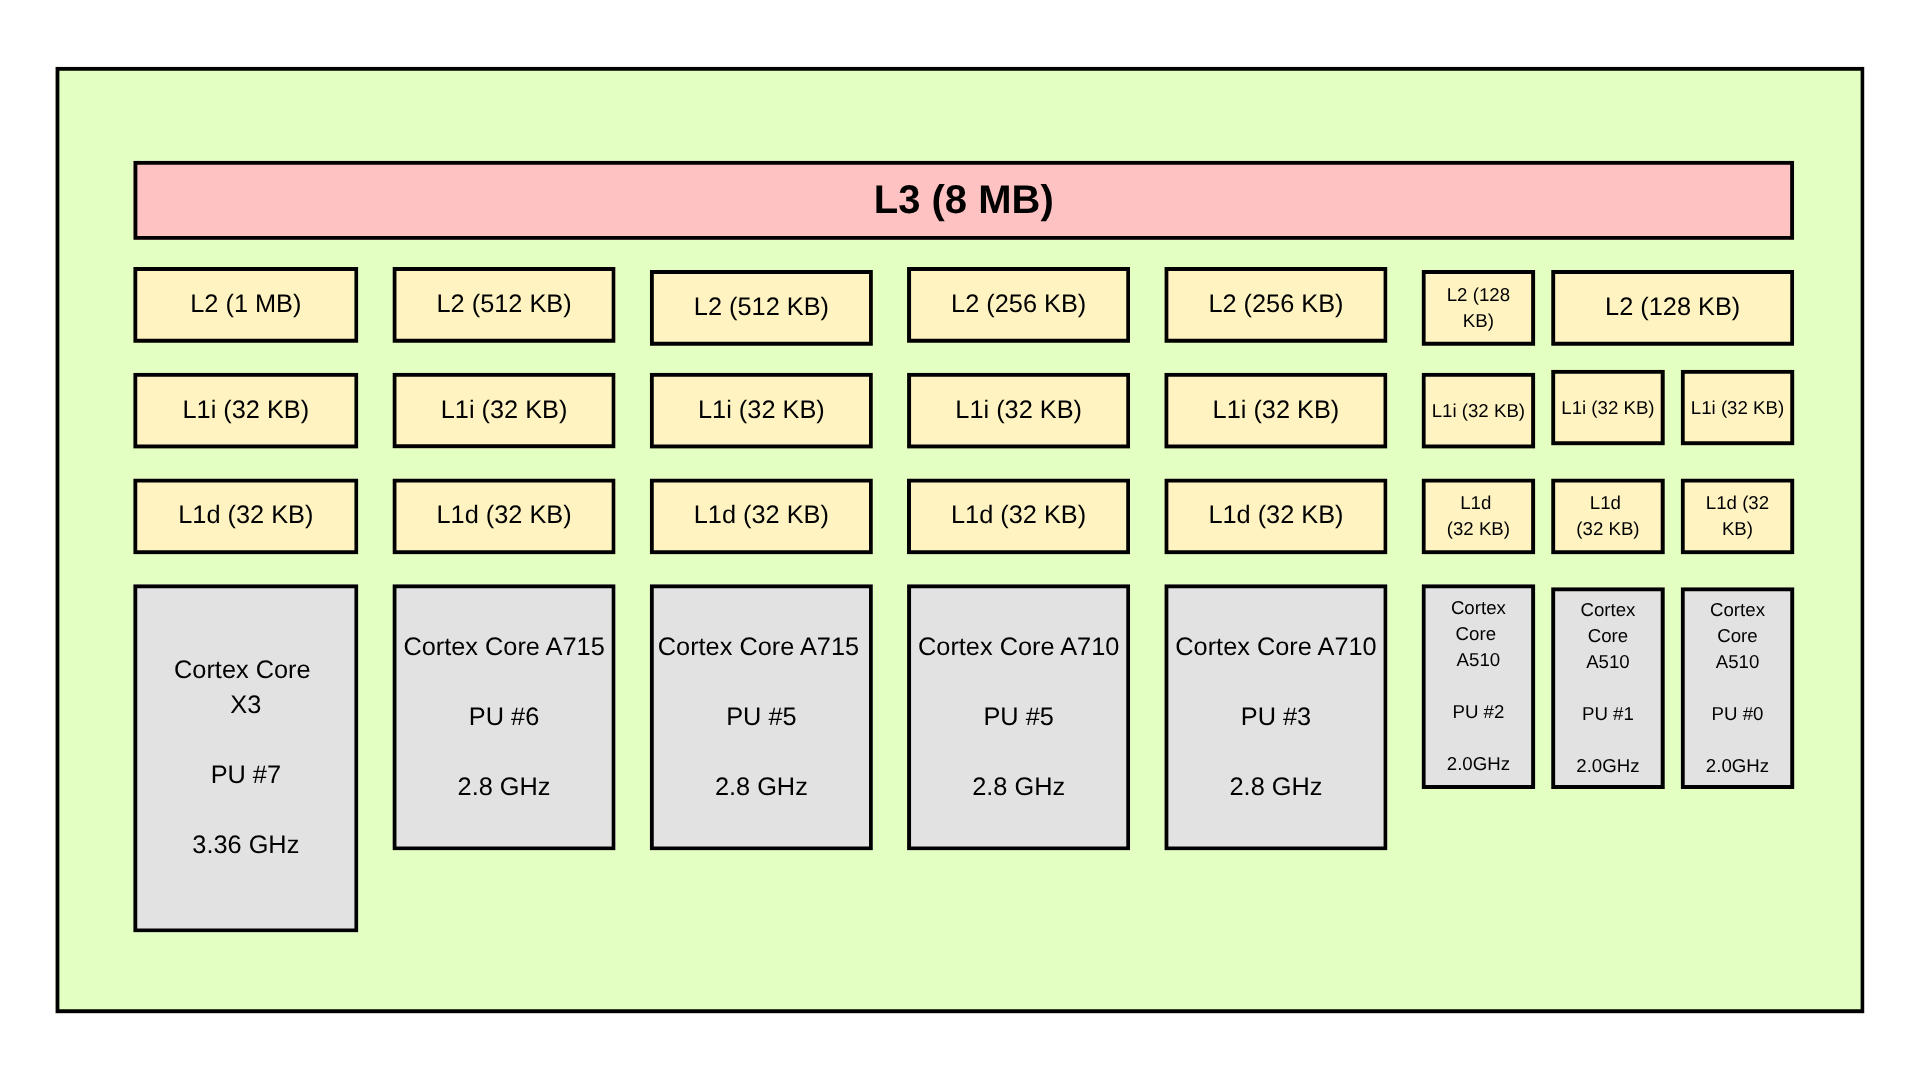
\includegraphics[width=0.8\textwidth]{assets/img/tabS9_arch.png}
    \caption{CPU topology of the Snapdragon 8 Gen 2 for Galaxy, showing the three tiers of cores and their cache hierarchy.}
    \label{fig:snapdragon}
\end{figure}
 
All cores share a single 8~MB L3 cache. This topology is representative of the heterogeneous big.LITTLE designs for which static work-sharing strategies are known to be ill-suited~\cite{alomairy2015numa}.
 
\subsection{Models and Workloads}
 
Two open-weight Transformer models are evaluated: \textbf{Llama-3.2-1B} (1.24 billion parameters, 32 decoder layers, GQA with 8 KV heads and 32 query heads, hidden dimension 2048) and \textbf{Qwen3-0.6B} (600 million parameters, 28 decoder layers, MQA-like GQA). Both models are run in float32 precision. Two sequence lengths are evaluated: a short context of 17 tokens and a longer context of 57 tokens, which increases the cost of the attention kernel and thus the degree of intra-iteration irregularity.
 
\subsection{Core Affinity Configurations}
 
Four CPU affinity masks are studied to isolate the effect of core heterogeneity:
 
\begin{itemize}
    \item \textbf{cpu\_7}: single-core (X3 prime only). Used as a sequential baseline; parallel experiments are not applicable.
    \item \textbf{cpu\_0\_2}: efficiency cores only (3$\times$ A510). Homogeneous, low-frequency cluster.
    \item \textbf{cpu\_3\_6}: performance cores only (2$\times$ A710 + 2$\times$ A715). Homogeneous high-frequency cluster.
    \item \textbf{cpu\_0\_7}: all 8 cores. The maximally heterogeneous configuration, exposing a 1.68$\times$ frequency ratio between the slowest (A510, 2.0~GHz) and fastest (X3, 3.36~GHz) core.
\end{itemize}
 
For cpu\_0\_7, the number of OpenMP threads is swept from 1 to 8. Thread $i$ is pinned to physical core P\#$i$ via \texttt{taskset}, so the composition of the active core set changes qualitatively as the thread count increases (see Section~\ref{sec:discussion}).
 
\subsection{Metrics}
 
Performance is reported in tokens per second (TPS) for both the \emph{prefill} phase (parallel processing of the input prompt) and the \emph{decode} phase (autoregressive generation, one token per forward pass). Each configuration is repeated 15 times and results are averaged. The speedup ratio $S = \text{TPS}_{\text{WS-on}} / \text{TPS}_{\text{WS-off}}$ quantifies the gain of the work-stealing scheduler over the OpenMP work-sharing baseline.
 
\section{Results and Discussion}
\label{sec:discussion}
 
\subsection{Static OpenMP Schedule: A Motivating Baseline}
 
Before analysing the main results, it is instructive to examine the performance of the work-stealing scheduler when deployed \emph{against the static OpenMP schedule}. This experiment — conducted with Qwen3-0.6B on the full 8-core heterogeneous platform (cpu\_0\_7), at 57 input tokens — constitutes the most compelling illustration of why heterogeneity-aware dynamic scheduling is essential for Transformer inference on big.LITTLE hardware.
 
The \texttt{schedule(static)} clause in OpenMP partitions the iteration space into equal-sized chunks and assigns them to threads at compile time, with no subsequent rebalancing~\cite{yanghe2018survey}. On a homogeneous multiprocessor this strategy incurs minimal overhead and achieves near-optimal load balance. On a heterogeneous platform such as ours, however, it is fundamentally ill-suited: a thread pinned to an A510 core (2.0~GHz) receives the same number of iterations as a thread pinned to the X3 prime core (3.36~GHz), yet requires $3.36/2.0 \approx 1.68\times$ more wall-clock time to complete them. The fast cores consequently stall at the implicit barrier at the end of each parallel region, waiting for the stragglers on efficiency cores, a phenomenon known as the \emph{straggler effect} as stated by Mishra and Nandivada~\cite{mishra2024cows}.
 
The results confirm this pathology dramatically. With the static schedule and \emph{no} work-stealing (\texttt{WS\_off}), the prefill throughput degrades from 39.9~TPS at 3 threads to only 14.7~TPS at 4 threads — a $2.72\times$ regression when a single A710 core is added to a homogeneous A510 cluster. This occurs because the fast A710 core receives a static chunk of equal size to the slow A510 cores, and then must idle until all three A510 threads complete; meanwhile the effective parallelism collapses to that of the slowest thread, effectively negating the benefit of the additional core.
 
The work-stealing scheduler eliminates this bottleneck entirely. With \texttt{WS\_on}, the fast cores steal the remaining iterations from slow cores as soon as they complete their initial (weighted) allocation, continuously keeping all cores productive as shown in figure~\ref{fig:static_schedule}.

\begin{figure}[H]
    \centering
    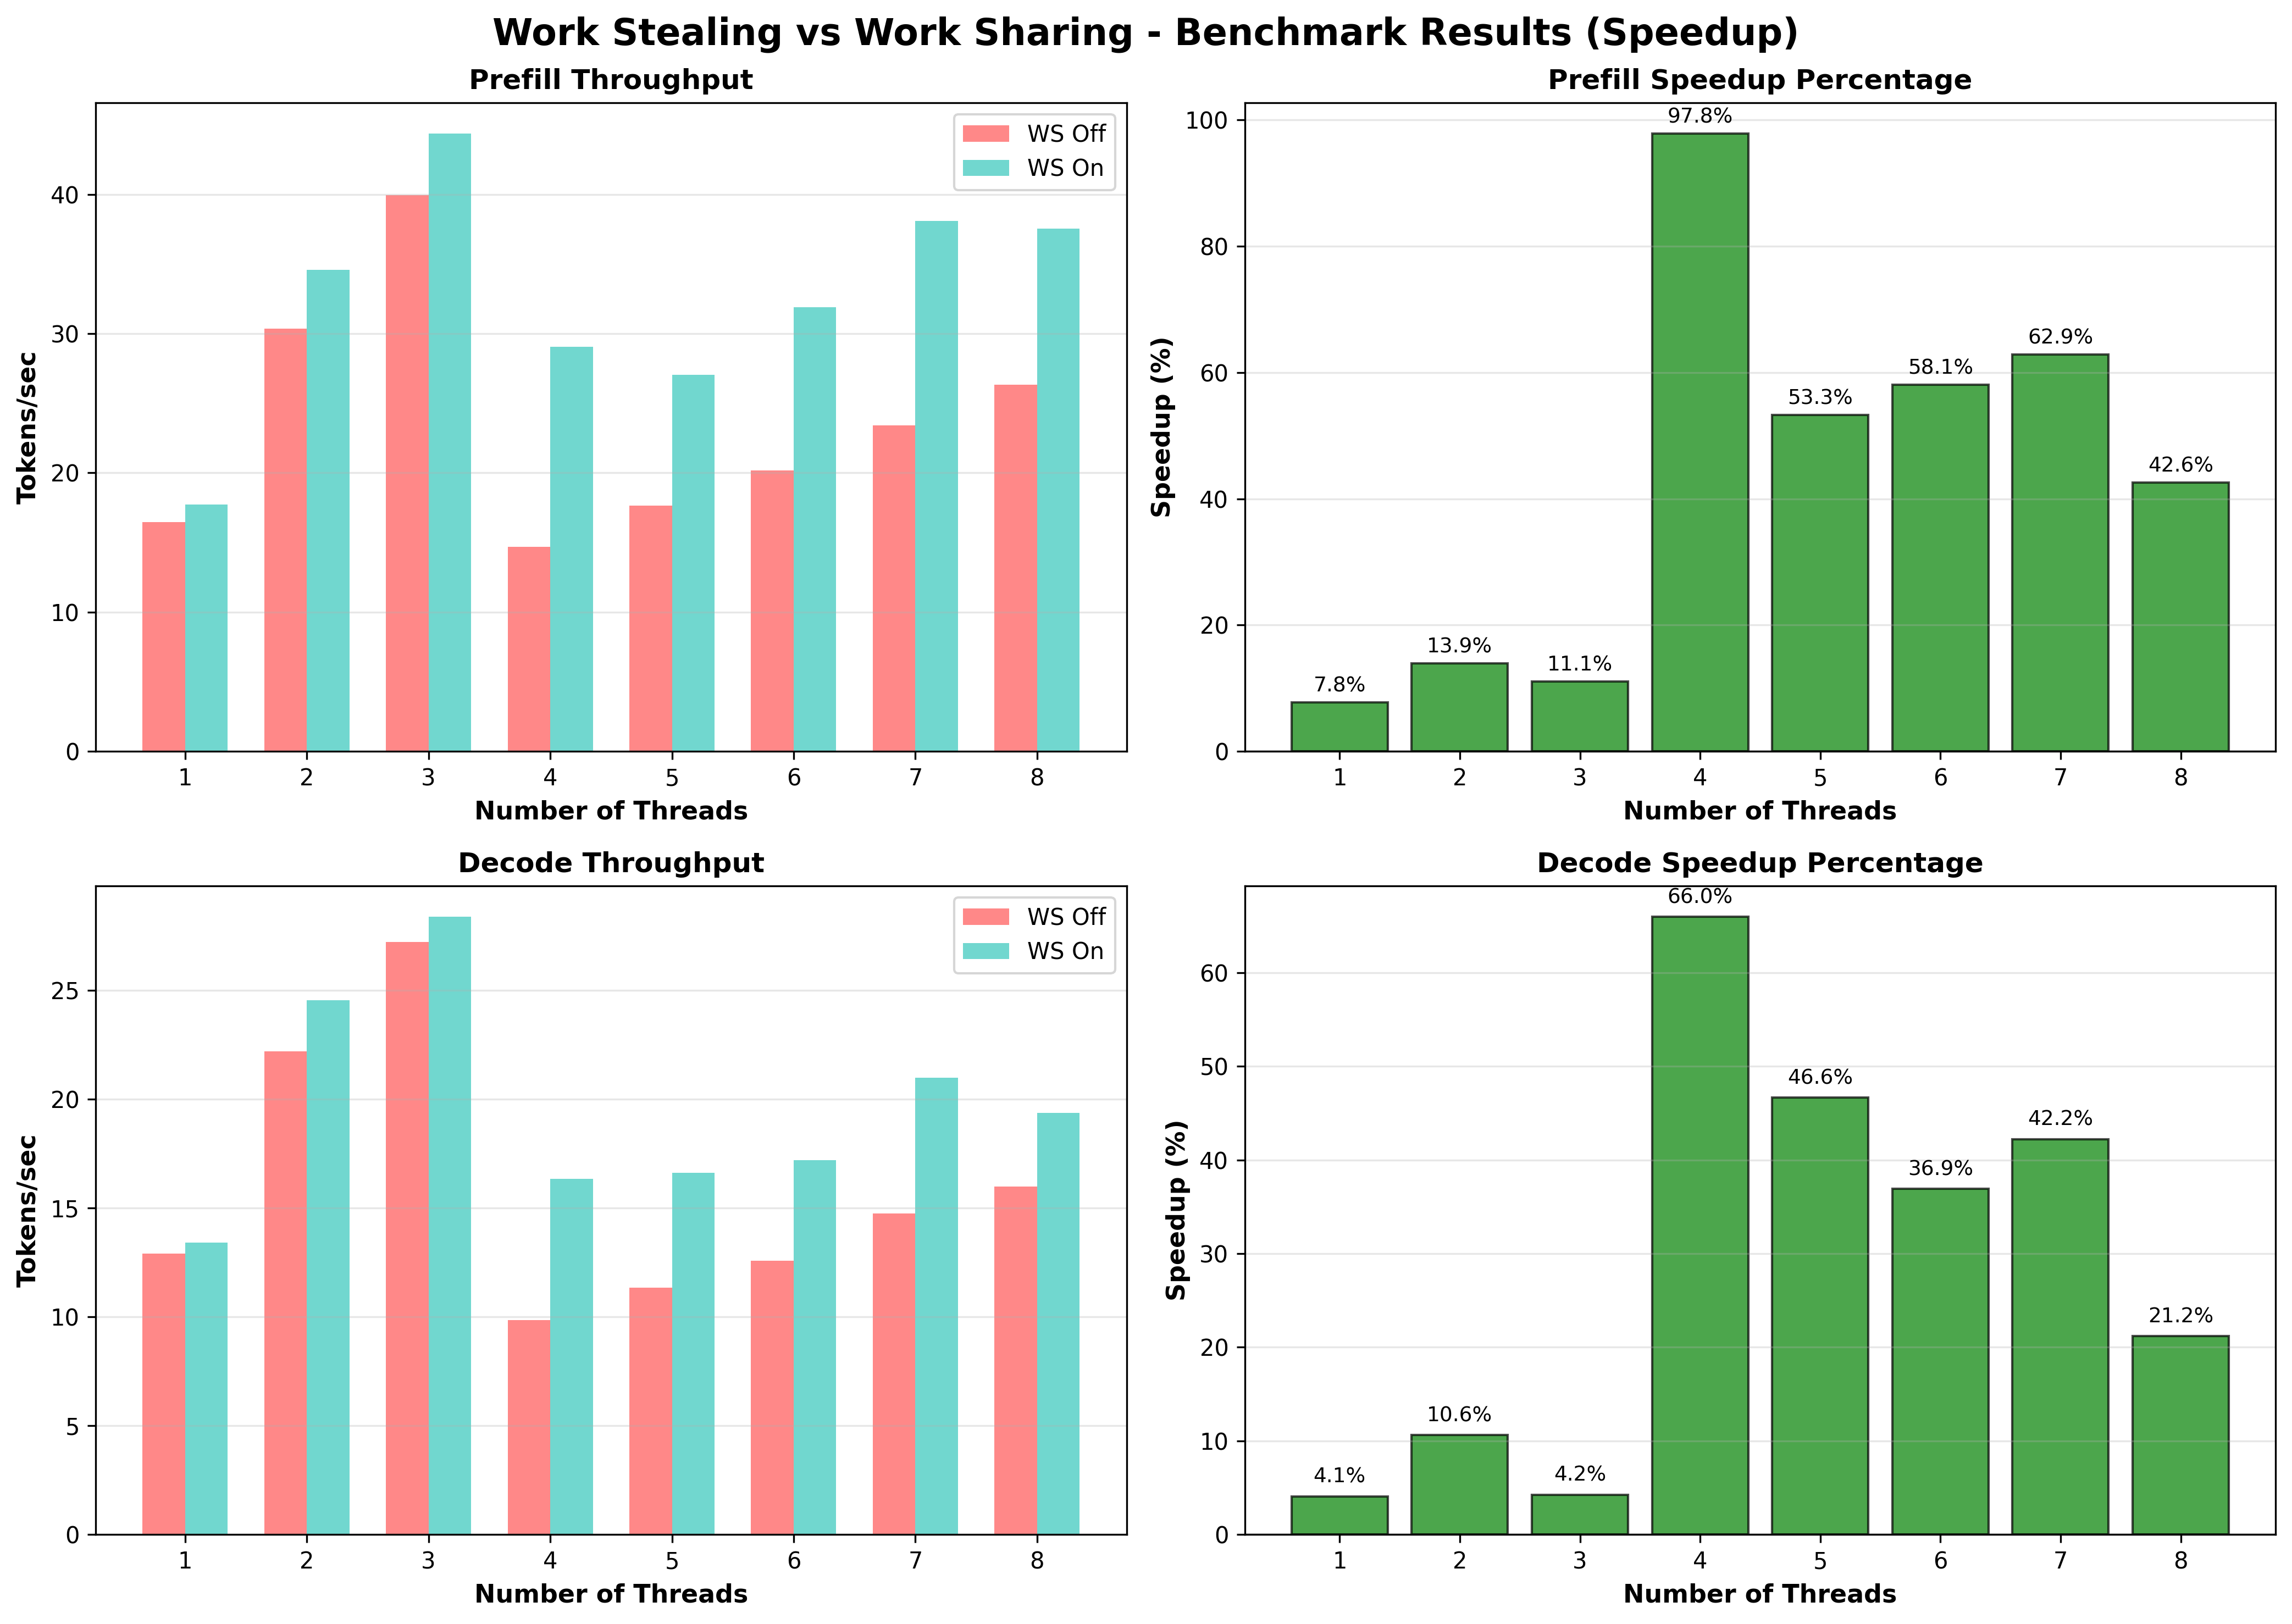
\includegraphics[width=0.8\textwidth]{assets/img/speedup_comparison_static.png}
    \caption{Benchmark results for Qwen3-0.6B at 57 input tokens, comparing the work-stealing scheduler against the static OpenMP schedule.}
    \label{fig:static_schedule}
\end{figure}
 
The decode phase shows striking improvements: up to $+65.96\%$ at 4 threads and $+46.64\%$ at 5 threads. These results confirm that, against a static schedule, work stealing is not merely beneficial — it is transformative. On heterogeneous hardware, the static schedule is a \emph{pathological} baseline, and any dynamic rebalancing mechanism will vastly outperform it. The work-stealing scheduler recovers nearly the full productive capacity of the heterogeneous cluster that a static schedule leaves stranded in idle stalls.
 
------
\subsection{Dynamic OpenMP Schedule: A More Competitive Baseline}
 
The remainder of the experiments compares the work-stealing scheduler against the OpenMP \texttt{schedule(dynamic)} clause, which is a significantly stronger baseline. Under \texttt{schedule(dynamic)}, a centralized task pool distributes individual iterations (or small chunks) to threads on demand: each idle thread fetches the next available chunk, so fast cores naturally acquire more iterations than slow ones over the course of execution. This achieves adaptive load balancing at the cost of (i) synchronization overhead on the shared task pool and (ii) reduced spatial locality, since iterations are no longer assigned contiguously to a single thread~\cite{yanghe2018survey}.

\subsection{Single Prime Core (cpu\_7): Scheduler Overhead in the Sequential Limit}
 
A degenerate but instructive configuration restricts execution to a single core: the Cortex-X3 prime core (P\#7, 3.36~GHz). With \texttt{OMP\_NUM\_THREADS=1}, no parallelism is exploited and no stealing can occur. This isolates the \emph{net overhead} of the OpenMP dynamic scheduling runtime from any actual parallelism benefit, and serves as a clean measurement of what the WS scheduler gains by eliminating that overhead.
 
The results are good: even with a single worker, the WS scheduler outperforms the OMP dynamic baseline by $+22$--$+28\%$ on decode and $+19$--$+28\%$ on prefill across both models (Table~\ref{tab:cpu7}).
 
\begin{table}[h]
\centering
\caption{Single-core (cpu\_7, Cortex-X3) throughput, decode TPS. WS-on vs.\ OMP dynamic.}
\label{tab:cpu7}
\begin{tabular}{llcccc}
\hline
Model & Steps & WS-off (TPS) & WS-on (TPS) & Speedup & Gain \\
\hline
Llama-3.2-1B & 17 & 1.243 & 1.540 & $1.239\times$ & +23.87\% \\
Llama-3.2-1B & 57 & 1.235 & 1.512 & $1.224\times$ & +22.41\% \\
Qwen3-0.6B   & 17 & 2.536 & 2.892 & $1.140\times$ & +14.00\% \\
Qwen3-0.6B   & 57 & 2.630 & 2.843 & $1.081\times$ & +8.11\%  \\
\hline
\end{tabular}
\end{table}

 
\subsubsection{Homogeneous Efficiency Cores (cpu\_0\_2)}
 
The first configuration (cpu\_0\_2) pins threads exclusively to the three Cortex-A510 cores (P\#0, P\#1, P\#2). All cores are frequency-identical (2.0~GHz), so load imbalance arises only from irregular iteration costs (i.e., the growing KV-cache in the attention kernel) rather than from hardware heterogeneity.
 
Under these conditions, the work-stealing scheduler consistently outperforms OpenMP dynamic across both models and both sequence lengths as figure~\ref{fig:cpu0_2} shows.

\begin{figure}[H]
    \centering
    
\includegraphics[width=0.49\textwidth]{\detokenize{assets/img/Qwen3-0.6B_cpu_0_2_steps_57.png}} % chktex 8
    
\includegraphics[width=0.49\textwidth]{\detokenize{assets/img/Llama-3.2-1B_cpu_0_2_steps_57.png}} % chktex 8
    \caption{Benchmark results for cpu\_0\_2 (3$\times$ A510 cores).}
    \label{fig:cpu0_2}
\end{figure}
 
 
The decode gain decreases monotonically with thread count, from $+21\%$ at 1 thread to $+6\%$ at 3 threads for Llama, and nearly vanishing ($+1\%$) for Qwen3 at 3 threads. Two effects compound here. First, as more workers participate, the OMP dynamic scheduler's per-iteration overhead is amortized over more threads, narrowing the WS advantage. Second, decode is inherently memory-bound: with batch size 1, each matmul loads model weights for a single token, resulting in arithmetic intensity well below the roofline threshold of even the A510 cores. Under such conditions, all threads are stalled waiting for L3 bandwidth, a shared resource, and any scheduling overhead is proportionally more costly relative to the compute saved~\cite{dice2021transformercpu}. The smaller Qwen3-0.6B model amplifies this effect further: its per-iteration compute is smaller, making the residual stealing overhead more visible at 3 threads.
 
\subsubsection{Homogeneous Performance Cores (cpu\_3\_6)}
 
The cpu\_3\_6 configuration restricts execution to cores P\#3--P\#6 (2$\times$ A710 and 2$\times$ A715 at 2.8~GHz). This is again a homogeneous cluster, but at a significantly higher clock frequency and with substantially more L2 cache per core (256--512~KB vs. 128~KB on A510), meaning less L3 pressure per thread.
 
Focusing on decode throughput at 57 tokens, the primary metric, the gains are consistent and positive across all thread counts as you can see in figure~\ref{fig:cpu3_6}.
 
\begin{figure}[H]
    \centering
    
\includegraphics[width=0.49\textwidth]{\detokenize{assets/img/Qwen3-0.6B_cpu_3_6_steps_57.png}} % chktex 8
    
\includegraphics[width=0.49\textwidth]{\detokenize{assets/img/Llama-3.2-1B_cpu_3_6_steps_57.png}} % chktex 8
    \caption{Benchmark results for cpu\_3\_6 (2$\times$ A710 + 2$\times$ A715 cores).}
    \label{fig:cpu3_6}
\end{figure}

 
These gains are notably more stable across thread counts compared to the efficiency-core cluster, and crucially there is \emph{no regression at 4 threads} unlike what is observed with shorter sequences (17 tokens) where the Llama decode regresses to $-2.37\%$ at 4 threads. This contrast is instructive: at 57 tokens, the attention kernel performs more work per task (the KV-cache contains more entries), providing the scheduler with a larger and more irregular workload to rebalance, which justifies the cost of the epoch barrier and atomic deque operations. At 17 tokens, the per-task work is so small that this overhead exceeds the load-balance gain.
 
The larger private L2 caches on A710/A715 cores (256--512~KB vs.\ 128~KB on A510) also contribute: the LIFO dequeue policy of the owner ensures high L2 reuse, and the stealing overhead is more easily absorbed against the higher compute throughput of these cores. The result is that on the homogeneous performance cluster at 57 tokens, the work-stealing scheduler provides a clean and consistent decode speedup with no pathological cases.
 
\subsubsection{Fully Heterogeneous Platform (cpu\_0\_7): The Critical Regime}
\label{sec:cpu07}
 
The cpu\_0\_7 configuration is the most revealing and the most challenging. With threads pinned sequentially to cores P\#0 through P\#$N-1$, the composition of the active core set changes qualitatively as $N$ increases:
 
\begin{itemize}
    \item \textbf{$N = 1$--$3$}: All threads on A510 cores (P\#0--P\#2). Homogeneous, efficiency cluster.
    \item \textbf{$N = 4$--$6$}: Mixed A510 + A710/A715. Heterogeneous cluster with slow (A510, 2.0~GHz) and fast (A710, 2.8~GHz) cores coexisting.
    \item \textbf{$N = 7$--$8$}: Full cluster including A715 cores and, at $N=8$, the X3 prime core (3.36~GHz).
\end{itemize}
 
This structure creates three qualitatively distinct performance regimes, each illuminating a different aspect of the scheduler's strengths and limitations.

\begin{figure}[H]
    \centering
    
\includegraphics[width=0.49\textwidth]{\detokenize{assets/img/Qwen3-0.6B_cpu_0_7_steps_57.png}} % chktex 8
    
\includegraphics[width=0.49\textwidth]{\detokenize{assets/img/Llama-3.2-1B_cpu_0_7_steps_57.png}} % chktex 8
    \caption{Benchmark results for cpu\_0\_7 (all 8 cores).}
    \label{fig:cpu0_7}
\end{figure}
 
\paragraph{Regime 1: $N = 1$--$3$ (homogeneous efficiency cluster).}
 
At 57 tokens, the work-stealing scheduler consistently outperforms OMP dynamic on decode throughput: gains range from $+4.43\%$ to $+8.70\%$ for Llama and from $+5.66\%$ to $+9.63\%$ for Qwen3 across 1--3 threads as the results in figure~\ref{fig:cpu0_7} show. These gains are smaller than those observed in the isolated cpu\_0\_2 configuration, which may reflect interference from the inactive performance cores: even when those cores are not assigned OMP threads, the Linux power management subsystem may throttle A510 clock frequencies to maintain thermal balance on the shared package, slightly reducing effective throughput in the full-chip configuration.
 
\paragraph{Regime 2: $N = 4$--$6$ (heterogeneous A510 + A710/A715). The Pathological Case.}
 
This is where the work-stealing scheduler exhibits its most significant flaw. At 4, 5, and 6 threads, \texttt{WS\_on} is systematically \emph{slower} than \texttt{WS\_off} across both models at 57 tokens. The decode regressions, the most operationally relevant metrics, are:
 
\begin{itemize}
    \item Llama-3.2-1B, 57 steps, 4 threads: $\mathbf{-9.34\%}$ decode ($-16.38\%$ prefill).
    \item Qwen3-0.6B, 57 steps, 5 threads: $\mathbf{-10.55\%}$ decode ($-11.60\%$ prefill).
    \item Qwen3-0.6B, 57 steps, 6 threads: $\mathbf{-17.33\%}$ decode ($-16.27\%$ prefill).
\end{itemize}
 
The decode regressions are particularly damaging because decode is already the bottleneck of autoregressive inference; making it $10$--$17\%$ slower than baseline is a meaningful degradation in user-visible latency.
 
We identify four compounding causes for this regression:
 
\textbf{(i) Range coarseness vs. fine-grained dynamic scheduling.} The work-stealing scheduler encodes the entire iteration space as \emph{one range per worker}. With $N=4$ threads, the scheduler creates 4 ranges and distributes them. A steal moves an entire range, this means there is no sub-division. By contrast, OMP \texttt{schedule(dynamic)} with default chunk size 1 distributes \emph{individual iterations} from a shared pool: a fast A710 core that finishes its current iteration immediately fetches the next, with no waiting. The effective rebalancing granularity of WS is thus $1/(N \cdot \text{ranges\_per\_worker}) = 1/4$ of the total work per steal, whereas OMP dynamic can redistribute at iteration-level granularity. When the total number of iterations per parallel region is moderate (e.g., 8 KV-heads $\times$ 57 tokens for the attention kernel), this coarseness means that a single steal may transfer far more work than necessary, resulting in the thief becoming the new straggler~\cite{mishra2024cows}.
 
\textbf{(ii) Inaccuracy of frequency-based weight estimation.} The scheduler assigns weights proportional to the CPU's maximum clock frequency. However, for memory-bound kernels (particularly decode, with batch size 1), the effective throughput ratio between an A510 and an A710 core is determined primarily by \emph{memory bandwidth}, not compute frequency. The A510 and A710 are both limited by L3 cache bandwidth, a shared resource, rather than their respective arithmetic units. The frequency-based weight map $\{1, 2, 4\}$ therefore overestimates the productive advantage of A710 over A510 for memory-bound workloads, causing the scheduler to under-provision the A510 cores and over-provision the A710 cores, leading to a systematic \emph{over-steal} from the A710 side~\cite{dice2021transformercpu,jiang2022arm}.
 
\textbf{(iii) Spinning overhead from fast-core idle stalls.} When an A710 or A715 core exhausts its (over-provisioned) work allocation ahead of the A510 threads, it enters the stealing loop, which spins on atomic loads of the \texttt{remaining} counters. These spinning operations generate sustained L3 coherence traffic (shared-line invalidations) that \emph{degrades the throughput} of the still-executing A510 threads by polluting the shared L3 with coherence requests. This is a well-documented pathology in work-stealing systems with heterogeneous processing rates~\cite{yanghe2018survey}: the idle fast cores, rather than being neutral, actively harm the slow cores' performance through cache interference.
 
\textbf{(iv) Epoch barrier overhead.} The epoch-based barrier requires all workers to reach a consistent state before and after each \texttt{ws\_for\_omp} invocation. At $N=4$--$6$ threads, the A510 cores are systematically the last to reach the end-of-epoch synchronization point, forcing the faster A710 threads to spin on the \texttt{threads\_done} counter. This spin introduces an additional serialization point that does not exist in OMP dynamic, whose implicit barrier uses a more efficient libgomp futex-based wait on Linux.
 
\paragraph{Regime 3: $N = 7$--$8$ (full heterogeneous cluster with A715 and X3).}
 
Paradoxically, the work-stealing scheduler recovers and outperforms OMP dynamic at 7 and 8 threads. At 57 tokens, the decode gains are:
 
\begin{itemize}
    \item Llama-3.2-1B, 7 threads: $\mathbf{+24.78\%}$ decode ($+21.27\%$ prefill).
    \item Llama-3.2-1B, 8 threads: $\mathbf{+18.93\%}$ decode ($+29.10\%$ prefill).
    \item Qwen3-0.6B, 7 threads: $\mathbf{+18.65\%}$ decode ($+16.31\%$ prefill).
    \item Qwen3-0.6B, 8 threads: $\mathbf{+18.37\%}$ decode ($+24.36\%$ prefill).
\end{itemize}
 
This recovery is attributable to a change in the \emph{dominant bottleneck}. At $N=7$--$8$, the OMP dynamic baseline (\texttt{WS\_off}) itself degrades noticeably compared to $N=6$: for Qwen3-0.6B at 57 steps, the decode baseline falls from 17.18~TPS at 6 threads to 12.36~TPS at 7 threads, despite gaining an additional high-performance A715 core. This is a strong indicator of \emph{OMP runtime contention}: the centralized task pool of OMP dynamic is implemented using a shared atomic counter (fetch-and-add) or a mutex-protected queue. At $N=7$--$8$ threads, contention on this shared structure grows super-linearly, causing the fast X3 and A715 cores to frequently stall at the task-fetch point, wasting their superior compute capacity on synchronization overhead~\cite{yanghe2018survey}.
 
The work-stealing scheduler, by contrast, is \emph{decentralized}: each thread operates on its own Chase--Lev deque and contacts other threads only when its local deque is exhausted. At high thread counts, this decentralized structure scales far better than a shared queue, which is the canonical theoretical justification for work stealing over work sharing~\cite{blumofe1999workstealing}. The gains at $N=7$--$8$ thus reflect the scheduler recovering the concurrency that the OMP runtime wastes on synchronization.
 
The X3 prime core (added at $N=8$) is assigned weight 4 by the frequency-tier mapping, giving it a proportionally large initial range. Its 1~MB private L2 cache allows it to sustain high arithmetic throughput on large iteration sub-ranges without L3 pressure, which further amplifies the WS advantage at full thread count.

 
\subsubsection{Effect of Sequence Length}
 
Comparing the 17-token and 57-token results reveals a consistent pattern: \emph{the decode speedup from WS tends to decrease with longer sequences}, while prefill speedups remain comparable. At 57 tokens, the attention kernel's KV-cache grows proportionally, increasing each task's cost and the total irregularity of the iteration space. One might expect this to benefit WS. However, with larger KV-caches, the memory footprint per attention task also grows, increasing L3 pressure. Under L3 saturation, the memory-bandwidth argument of point (ii) above becomes even more dominant: the frequency-based weight function remains inaccurate, and the steal granularity remains coarse. The benefit of dynamic rebalancing is therefore not amplified by longer sequences in the way that a finer-grained work-stealing implementation (e.g., with recursive range splitting) would achieve.
 
\subsection{Summary of Findings}
 
The experimental results highlight a clear dichotomy in the scheduler's behaviour:
 
\begin{itemize}
    \item Against \texttt{schedule(static)}, the work-stealing scheduler is unambiguously superior, delivering up to $+97.83\%$ prefill improvement by eliminating the straggler effect that static scheduling induces on heterogeneous big.LITTLE hardware.
    \item Against \texttt{schedule(dynamic)}, the work-stealing scheduler wins decisively on homogeneous clusters and at high thread counts ($N \geq 7$), where OMP dynamic's centralized queue becomes the bottleneck. It loses in the mixed-core regime ($N = 4$--$6$) due to coarse steal granularity, inaccurate heterogeneity weight estimation, and spinning-induced L3 interference from idle fast cores.
\end{itemize}
 
The root cause of the regressions at $N=4$--$6$ is the mismatch between the scheduler's \emph{range-based task model} (one steal per initial allocation) and the fine-grained dynamic demand of a heterogeneous platform where the performance differential between A510 and A710 cores is irregular and workload-dependent. Future work should investigate adaptive range splitting (recursive halving when a range is stolen) and bandwidth-aware weight functions to address these limitations.

\section{Conclusion}

\bibliographystyle{alpha}
\bibliography{assets/sched-ter}

\end{document}
